%-----------------------------------------------------------------------------
%
%               Template for LaTeX Class/Style File
%
% Name:         sigplanconf-template.tex
% Purpose:      A template for sigplanconf.cls, which is a LaTeX 2e class
%               file for SIGPLAN conference proceedings.
%
% Author:       Paul C. Anagnostopoulos
%               Windfall Software
%               978 371-2316
%               paul@windfall.com
%
% Created:      15 February 2005
%
%-----------------------------------------------------------------------------


\documentclass[preprint,natbib]{sigplanconf}

\usepackage{amsmath}
\usepackage{amsfonts}
\newcommand{\mt}[1]{\mbox{\it #1}}
\newcommand{\todo}[1]{
    \addcontentsline{tdo}{todo}{\protect{#1}}
    \marginpar{#1}
}

\begin{document}

\conferenceinfo{PLDI '09}{June 2009, Dublin, Ireland.} 
\copyrightyear{2009} 
\copyrightdata{[to be supplied]} 

\titlebanner{Submitted for confidential review to: ACM SIGPLAN 2009 Conference on 
Programming Language Design and Implementation (PLDI)}

\title{Data-Parallelization of Sliding-Window Computations\\in Stream Programs}

\authorinfo{Anonymous}
           {}
           {}
%\authorinfo{Name2\and Name3}
%           {Affiliation2/3}
%           {Email2/3}

\maketitle

\begin{abstract}
Due to the high data rates involved in audio, video, and signal
processing applications, it is imperative to compress the data to
decrease the amount of storage used.  Unfortunately, this implies that
any program operating on the data needs to be wrapped by a
decompression and re-compression stage.  Re-compression can incur
significant computational overhead, while decompression swamps the
application with the original volume of data.

In this paper, we present a program transformation that greatly
accelerates the processing of compressible data.  Given a program that
operates on uncompressed data, we output an equivalent program that
operates directly on the compressed format.  Our transformation
applies to stream programs, a restricted but useful class of
applications with regular communication and computation patterns.  Our
formulation is based on LZ77, a lossless compression algorithm
utilized by ZIP, and immediately applies to simpler formats such as
Apple Animation, Microsoft RLE, and Targa.

We implemented a simple subset of our techniques in the StreamIt
compiler, which emits executable plugins for two popular video editing
tools: MEncoder and Blender.  For common operations such as color
adjustment and video compositing, computing directly on compressed
data offers a speedup roughly proportional to the overall compression
ratio.  For our benchmark suite of 12 videos in Apple Animation
format, speedups range from 1.1x to 471x, with a median of 15x.

\end{abstract}

%\category{CR-number}{subcategory}{third-level}

%\terms
%term1, term2

%\keywords
%keyword1, keyword2

\section{Introduction}


Stream computing represents an increasingly important class of
applications. In streaming codes, there is an abundance of parallelism that
is easier to extract compared to traditional desktop workloads (e.g.,
pointer-based computing). As a result, the extraction of parallelism
in streaming codes does not require heroic efforts, and thus,
processors can deliver higher performance with significantly lower
power costs. This is especially important since
leading microprocessor companies have realized that modern general
purpose architectures are near their  performance limits for  the
amount of power they consume. Thus, the future will place a greater
emphasis on exploiting the properties of streaming workloads in
conventional von~Neumann architectures.

Streaming is a model of computation that uses sequences of data
and computation kernels to expose concurrency and locality for
efficiency~\cite{wss}. In general purpose processors, improving locality 
translates to an effective management of the memory hierarchy at all
levels, including the register file. In this paper, we present a
methodology for compiling streaming codes to general purpose,
cache-based architectures. We first introduce a simple model for
reasoning effectively about the caching behavior of streaming
workloads. This model serves as a foundation for several {\it cache-aware
optimizations} that are geared toward the concomitant increase of instruction
and data {\it temporal locality}. These
optimization lead to significantly better utilization of the memory
system, and as such, they deliver performance gains ranging from 11
to 99\% for our streaming benchmark suite.

The context for our work is StreamIt, an architecture-independent
language that is engineered for streaming
applications~\cite{streamitcc}. It adopts the 
Cyclo-Static Dataflow~\cite{BELP96} model of computation which is a
generalization of Synchronous Dataflow~\cite{LM87-i} (SDF).  
SDF is a popular  model that  is well suited for
streaming codes. In SDF, computation is represented as a graph
consisting of {\it  actors} connected by communication channels; the
actors consume  and produce a constant number  of items from their
input and output  channels every time they execute. SDF is appealing
because it is amenable to static scheduling and optimization. 

From a general purpose architecture's point of view, actors represent
computation kernels, and the communication between actors represents
data buffers that must be streamed to and from the processor. Thus
the size of an actor and the
order of actor executions are critical properties that
impact the performance of the instruction cache. For example, the
compiler must make sure the actor's code size is not
greater than the instruction cache. Furthermore, we must {\it scale}
the execution of the actor so that it runs several times before we move
on to some other actor in the stream 
graph. This serves to $(i)$ amortize the cost of fetching the actor's
instructions into the cache from memory (an expensive operation), $(ii)$
improve the instruction temporal locality, and $(iii)$ improve overall
performance. However, as our cache model will show, we 
cannot arbitrarily scale the execution frequency of an actor. This
is because actors produce data that must be buffered, and therefore,
we must also consider the amount of data an actor produces and
consumes if we are to adequately manage the data cache. This paper is unique
in that it is the first to present a unified optimization methodology
that simultaneously considers instruction and data locality for
mapping streaming computation to cache-based architectures.

In terms of improving the data cache behavior, the compiler schedules
actor firing such that the producer-consumer locality is
preserved. Furthermore,  the compiler may {\it fuse}
together two or more actors to form a coarser grained kernel.
The fusion allows for better register allocation as we can
destroy the arrays used to buffer data between the actors and replace
the corresponding array references with scalars.  It also allows for
various competing implementations for managing the buffers between the
fused actors.  This paper evaluates several implementation
alternatives (for buffer management) and evaluates their performance.

The methodology for fusing actors leverages a distinguishing StreamIt
characteristic, namely, the hierarchical organization of
the stream graph. Furthermore, the algorithm for fusing actors applies
for the various topologies allowed by StreamIt.
It also considers another distinguishing characteristics of StreamIt,
namely the {\tt peek} operation whereby an actor may inspect data
items in its input buffer without consuming them until some future
execution. While peeking is a powerful language feature, it does pose
some challenges to the compiler and the cache optimizations. Peeking
also impacts the choice for the best buffer management strategy, as our
study will show.

%% the comment about p3 and itanium not being embedded architectures
%% is out of the blue! need a better transition.
Cache-aware fusion alone delivers significant performance gains, although our
evaluation shows that fusion with scaling leads to the best
performance on a general purpose, cache-based architecture. For our
experiments, we use two different processors: a superscalar out-of-order
processor, and an in-order VLIW processor. The former is a Pentium~3
whereas the latter is an Itanium~2. While these architectures are not
particularly suited for an embedded system, they do exhibit some
properties that are worthy of investigation. Furthermore, that we can
demonstrate measurable performance gains on real systems is far more
convincing than using a simulation-based environment. We chose the
Pentium~3 processor because it has very few registers in its
instruction set architecture. The Itanium by contrast has a much 
larger and richer repertoire of registers. The two architectures serve
to validate our cache-aware optimizations, in that we expect an
architecture with more register to benefit more from optimization such
as scalar replacement. On average, fusion leads to a 47\% improvement
on the Pentium~3, and 50\% on the Itanium~2.

The two architectures also differ in terms of their memory system
organization. The Itanium is an in-order VLIW processor and does not
tolerate a memory stall as well as its out-of-order
counterpart. Therefore we expect different gains from the scaling
optimization which amortize the long access latencies for instruction
and data caches. On average, scaling leads to a 21\% improvement on
the Itanium~2, and 17\% on the Pentium~3.

While both scaling and fusion lead to modest performance gains, we
must combine the two to deliver the best possible performance. When we
do so, we can further improve the performance of our benchmarks by
53\% on average for the Pentium~3, and 55\% for the Itanium~2.

\subsection{Summary of Contributions}

This paper makes the following contributions:
\begin{itemize}

\item A cache model for stream computing that provides a quantitative
estimate of the caching performance for any sequence of actor
executions.

\item A cache-aware scheduling heuristic that judiciously increases
the multiplicity of actors, improving instruction and data locality
while not exceeding the data cache.

\item A cache-aware partitioning policy that judiciously fuses
adjacent actors into a single component, enabling local optimizations
while not exceeding the instruction cache.

\item An optimized buffer management policy, termed ``copy-shift with
execution scaling'', which out-performs a traditional rotating buffer
in a detailed micro-benchmark analysis.

\item A fully automatic implementation of the above techniques in the
StreamIt compiler.

\item An experimental evaluation across 11 streaming benchmarks,
demonstrating performance improvements of up to 99\%.
\end{itemize}

\subsection{Paper Roadmap}

The remainder of the paper is organized as follows. Section~\ref{sec:streamit}
describes StreamIt and introduces our motivating example.
Section~\ref{sec:cache-model} introduces our cache model for 
reasoning about the performance of a streaming
computation. Section~\ref{sec:cache-opt} describes our cache-aware
optimizations, and Section~\ref{sec:buffer} describes the 
optimization enabled by fusion. Section~\ref{sec:evaluation} describes
our evaluation methodology and present our experimental
analysis. Sections~\ref{sec:related-work}~and~\ref{sec:conclusion}
discuss related work and concludes the paper.

\section{Streaming Execution Model}

In order to rigorously describe our techniques it is necessary to
define an execution model for streaming computation. The model we use
for this paper is a general model that is agnostic of input language.

Consider a directed acyclic graph $G = (V, E)$ corresponding to a
streaming application. $F \in V$ is a filter in the application and
$(f, g) \in E$ is an edge in the graph that denotes communication from
$f$ to $g$ using a FIFO channel.  A filter may have multiple incoming
edges and multiple outgoing edges.  Filter inputs are organized into a
single FIFO buffer for the filter to read according to an {\it input
distribution pattern}, and filter outputs are distributed from an
output FIFO buffer according to a {\it output distribution pattern}.  Both
are described below.

One execution of a filter is termed a filter {\it firing}. For each
filter $F \in V$ a {\it prework} function, $W_p(F)$, and a {\it work},
$W(F)$ function is defined.  The prework function is executed on the
first firing of the filter and the work function is executed on all
subsequent firings of the filter.  These work functions are the atomic
unit of computation for a filter and denote a function with the
variable $\mathcal{F} \in \{W_p, W\}$.  In the work and prework
functions, a filter accesses its input tape via the expressions {\tt
pop()}, which dequeues and item, and {\tt peek(i)}, which inspects but
does not dequeue the item at index {\tt i} from the beginning of the
buffer (beginning at 0).  {\tt push(val)} enqueues an item onto the
output buffer.

For each filter $F \in V$ we define the following:
\begin{itemize}

\item $o(\mathcal{F}, F)$, the number of items dequeued from $F$'s
input buffer per firing of $\mathcal{F}$,

\item $e(\mathcal{F}, F)$, the number of items read (but not dequeued)
from $F$'s input buffer per firing of $\mathcal{F}$,

\item $u(\mathcal{F}, F)$, the number of items enqueued to $F$'s
output buffer per firing of $\mathcal{F}$,

\end{itemize}

For all $F \in V$, we require that the above quantities be statically
determinable.  Also, we require that the input and output distribution
patterns be statically determinable.  This special case of streaming
computation is termed synchronous dataflow (SDF) and it is natural and
expressive for many domains including DSP, network, image, voice, and
multimedia~\cite{leeSDF}.  Furthermore, applications with dynamic
I/O rates can often be cut into static rate region for which the
techniques in this paper are applicable~\cite{chen:graphics-hardware:2005}.

A schedule of a graph $G$ gives a multiplicity for each filter $F \in
V$ that denotes how many times to fire filter $F$. In the SDF domain,
a {\it steady-state} schedule, $S$, of a graph can be calculated such
that the quantity of items on each of the filter's input buffer and
output buffer remains unchanged by the complete execution of the
schedule~\cite{lee87}.  Thus this schedule can be repeated
indefinitely because buffers to not grow or shrink in size.
Furthermore, because of the {\tt peek} construct, a separate {\it
initialization} schedule, $I$, is required. After the initialization
schedule executes, each filter is guaranteed to have at least $e(W,
F)$ items in its input buffer. The initialization schedule is required
to calculate a steady-state schedule for a graph with an $F$ such that
$e(W, F) > 0$~\cite{karczmarek:lctes:2003}.  During application
execution, The initialization schedule is executed once followed by an
infinite repetition of the steady-state schedule. 

The number of items remaining on a $F$'s input buffer after execution
of the initialization schedule is given by $C(F)$. A schedule of
execution is denoted by the variable $\Sigma$, where $\Sigma \in
\{I, S\}$.  The multiplicity of filter $F$ in schedule $\Sigma$ is
denoted by $M(\Sigma, F)$.

The input distribution pattern for filter $F$ for schedule $\Sigma$ is
a weighted round-robin described by two sequences:

\[ \mt{IW}(\Sigma, F) \in (\mathbb{N}^{*})^n \]

\[ \mt{IE}(\Sigma, F) \in E^n \]
 
Conceptually, to gather the items on the multiple input edges for $F$
into $F$'s input buffer, we cycle through the edges $e_i \in
\mt{IE}(\Sigma, F)$ and wait for $w_i \in \mt{IW}(\Sigma, F)$ items
from $e_i$ to arrive on the edge, enqueuing each onto the input buffer.

The output distribution pattern describes both duplication and
distribution in the same structures. For filter $F$ and for schedule
$\Sigma$, the distribution is given by a sequence of weights and
sequence of sets of edges:

\[ \mt{OW}(\Sigma, F)  \in (\mathbb{N}^{*})^m \]

\[ \mt{OE}(\Sigma, F) \in (D_1, D_2, ..., D_m)  \mbox{ where }  D_i \subset
E \]

Each set $D_i$ of the outgoing edges denotes a duplication set of
edges. To scatter the items produced by a filter, we cycle through the
sets $D_i \in \mt{OE}(\Sigma, F)$ duplicating the item produced by $F$
to each of the edges $e \in D_i$. Each $D_i$ duplicates $w_i \in
\mt{OW}(\Sigma, F)$ output items from $F$ before moving on to
$D_{i+1}$.


\section{Fission of a Single Input / Single Output Filter}
\label{sec:single}

In this section we introduce our techniques by defining the
process of fission on a filter with a single input and a single
output. Portions of this process will be used for the more general
techniques discussed in Section~\ref{sec:general}. 

Given a stateless filter $F \in V$ and a fission factor $P$, we will
data-parallelize $F$ by creating $P$ modified copies of the filter
$F_1, ..., F_P$.  Each copy is constructed to execute an equal
percentage firings of $F$ in $S$.  The initialization stage is handled
in a special manner.  If $F$ executes in $I$ (i.e., $M(I,F) > 0$),
then our transformation constructs $F_1$ such that it performs all the
computation and data distribution of $F$ in $I$. $F$ has a single
incoming edge ${U,F}$ and a single outgoing edge ${F, D}$.

\todo{Figure showing the transformation}

We make the following assertions on $F$:

\begin{enumerate}

\item $M(S,F) \mod  P = 0$

\item $C(F) < O(S,F) \times M(S,F)$

\item $M(S,F) \times O(S,F) \ge 2(e(S,F) - o(S,F))$

\end{enumerate}

\todo{Discuss these more!}

\subsection{Initialization Stage Construction}

For the initialization stage the transformation defines the following,
where $1 < x \le P$. First, the initialization
schedule multiplicity and rates of filter $F_x$ are set to zero
because they are not involved in this stage:
$$ M(I,F_x) \equiv o(W_p,F_x) \equiv u(W_p,F_x) \equiv e(W_p,F_x)
\equiv 0 $$
$$ M(I,F_1) \equiv 1 $$

Next we define the properties of $F_1$ in the initialization stage. In
the transformation, $W_P(F_1)$ is constructed to execute all of the
firings of $F_1$ from $I$ in a single firing.  First $W_P(F)$ is
called once, and $W(F)$ is executed $M(I,F) - 1$ times:

\begin{algorithm}
$W_P(F_1)$:
\begin{algorithmic}[1]
\State $W_P(F)$
\For{$M(I,F) - 1$}
\State $W(F)$
\EndFor
\end{algorithmic}
\end{algorithm}

The rates in $I$ of $F_1$ are as follows:
 
\begin{eqnarray*} 
o(W_p,F_1) & \equiv & o(W_p,F) + [(M(I,F) - 1) \times o(W,F)] \\
e(W_p,F_1) & \equiv & \max(e(W_p,F), o(W_p,F_1) + e(W,F)) \\
u(W_p,F_1) & \equiv & u(W_P,F) + [M(I,F - 1) \times u(W_P,F)]
\end{eqnarray*} 

\begin{eqnarray*}
\mt{IW}(I,F_1) & \equiv & (1) \\
\mt{IE}(I,F_1) & \equiv & (\{U,F_1\}) 
\end{eqnarray*}

\begin{eqnarray*} 
\mt{OW}(I,F_1) & \equiv & (1) \\
\mt{OE}(I,F_1) & \equiv & ((\{F_1, D\})) 
\end{eqnarray*} 

\subsection{Steady-State Construction}
Define the following: $1 \le i \le P$.
 
$$ M(S,F_i) \equiv 1 $$

\begin{eqnarray*} 
o(W,F_i) & \equiv & \frac{M(S,F)}{P} \times o(W,F) + e(W,F)\\
e(W,F_i) & \equiv & 0 \\
u(W,F_i) & \equiv & \frac{M(S,F)}{P} \times u(W,F)
\end{eqnarray*} 

\begin{algorithm}
$W(F_i)$:
\begin{algorithmic}[1]
\For{$M(S,F)/P$}
\State $W(F)$
\EndFor
\State {\tt pop(}$e(W,F)${\tt)}
\end{algorithmic}
\end{algorithm}


\section{General Fission Technique}
\label{sec:general}

This section describes fission on a general filter with an arbitrary
number of inputs and outputs.  This section builds upon the techniques
discussed in Section~\ref{sec:single}. j
\section{Evaluation}
\label{sec:eval}

In this section we evaluate the framework presented in this paper.  We
have implemented the techniques in the context of the StreamIt
compiler infrastructure~\cite{gordon-asplos06}.  The fission and
sharing reduction techniques are guided by the parallelization
management algorithms covered in~\cite{gordon-asplos06}.  These
algorithms offer a holistic approach to exploiting coarse-grained
task, data, and pipeline parallelism.   Once, the parallelization management
algorithm decides how to exploit data-parallelism, i.e., which
filters should be data parallelized and by what degree, our fission
algorithm of Section~\ref{sec:data-par} is utilized to perform the
data-parallelization. 

We compare our techniques to previously published techniques for
fission of sliding window filters that perform duplication of all
input items and decimation of unneeded items (DupDec).  We employ
three benchmarks for the evaluation.  The ChannelVocoder benchmark is
the analyzer portion of a source-filter model speech coder.  The
Filterbank benchmark implements a multi-rate signal decomposition
processing block common in communications and image processing.  The
FMRadio benchmark implements an FM radio with multi-band equalizer.
The following table provides more details on the benchmarks:


{\centering
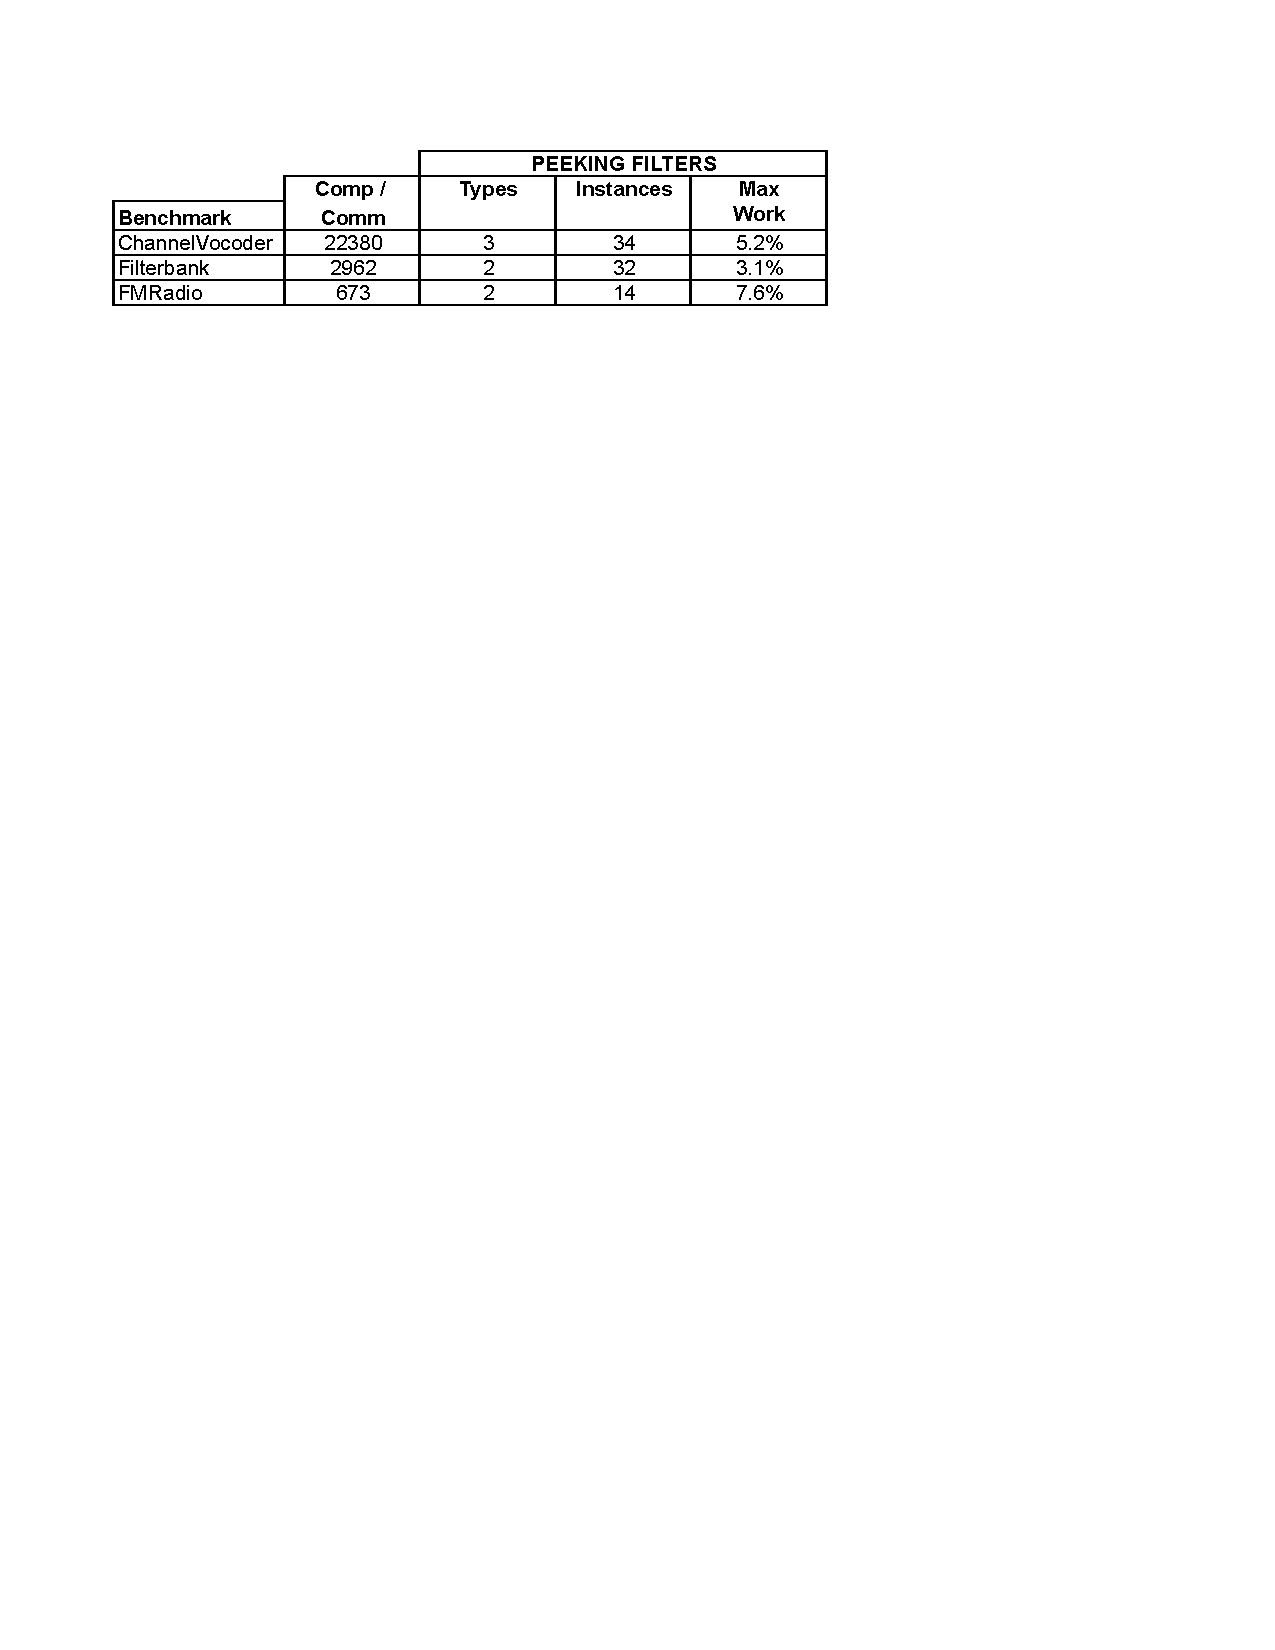
\includegraphics[width=3.3in]{figures/bench-char.pdf}}

\noindent ``Comp/Comm'' provides a static estimation of the
amount of computation to communication ratio by statically estimating the total
work of all the filters and dividing by the number items communicated
for the programmer-conceived graph's steady-state.  The remaining
statistics give the number of peeking filters types, number of peeking
filters instantiated at runtime, and a static estimation of the maximum
work in the single most loaded peeking filter.

We target 2 multicore architecture with different communication
mechanisms.  The Tilera Corporation's TILE64 Processor is a 64 core
system on a chip~\cite{tilera}.  Each core is an identical three-wide
VLIW. The code generated by the StreamIt
compiler for the TILE64 processor follows the remote store programming
(RSP) model~\cite{rsp10} in which each process has a private address
space, but each process can award remote processes write access to
their local memory. When a producer process has write access to a
consumer process's memory, the producer communicates directly with the
consumer via store instructions whose destination is an address in the
consumer's shared memory.  Communication is initiated by the producer,
and is fine-grained.  The consumer reads directly from it's local
memory (L2) when accessing input.

Our symmetric multiprocessor target is a 16-core architecture that is
comprised of four Intel Xeon E7350 multicore processors.  Each processor
is a 64-bit, quad-core with two dual-core dies.  Each die contains a 4
MB L2 cache shared across the two cores.  The front-side bus is clocked
at 1066 MHz.  We utilize the cache coherency mechanism of the
architecture for communication between cores. 

Through empirical experimentation on FMRadio, Filterbank, and
ChannelVocoder, we have settled on $T_{\mt{sharing}} =.10$ and
$T_{\mt{apply}} = 0.05$. These constants are the sweet stop for the two
architectures employed in the experimentation, being a good compromise
between buffer size and inter-core communication.

% \begin{figure*}[t]
% \centering
% \subfigure[]{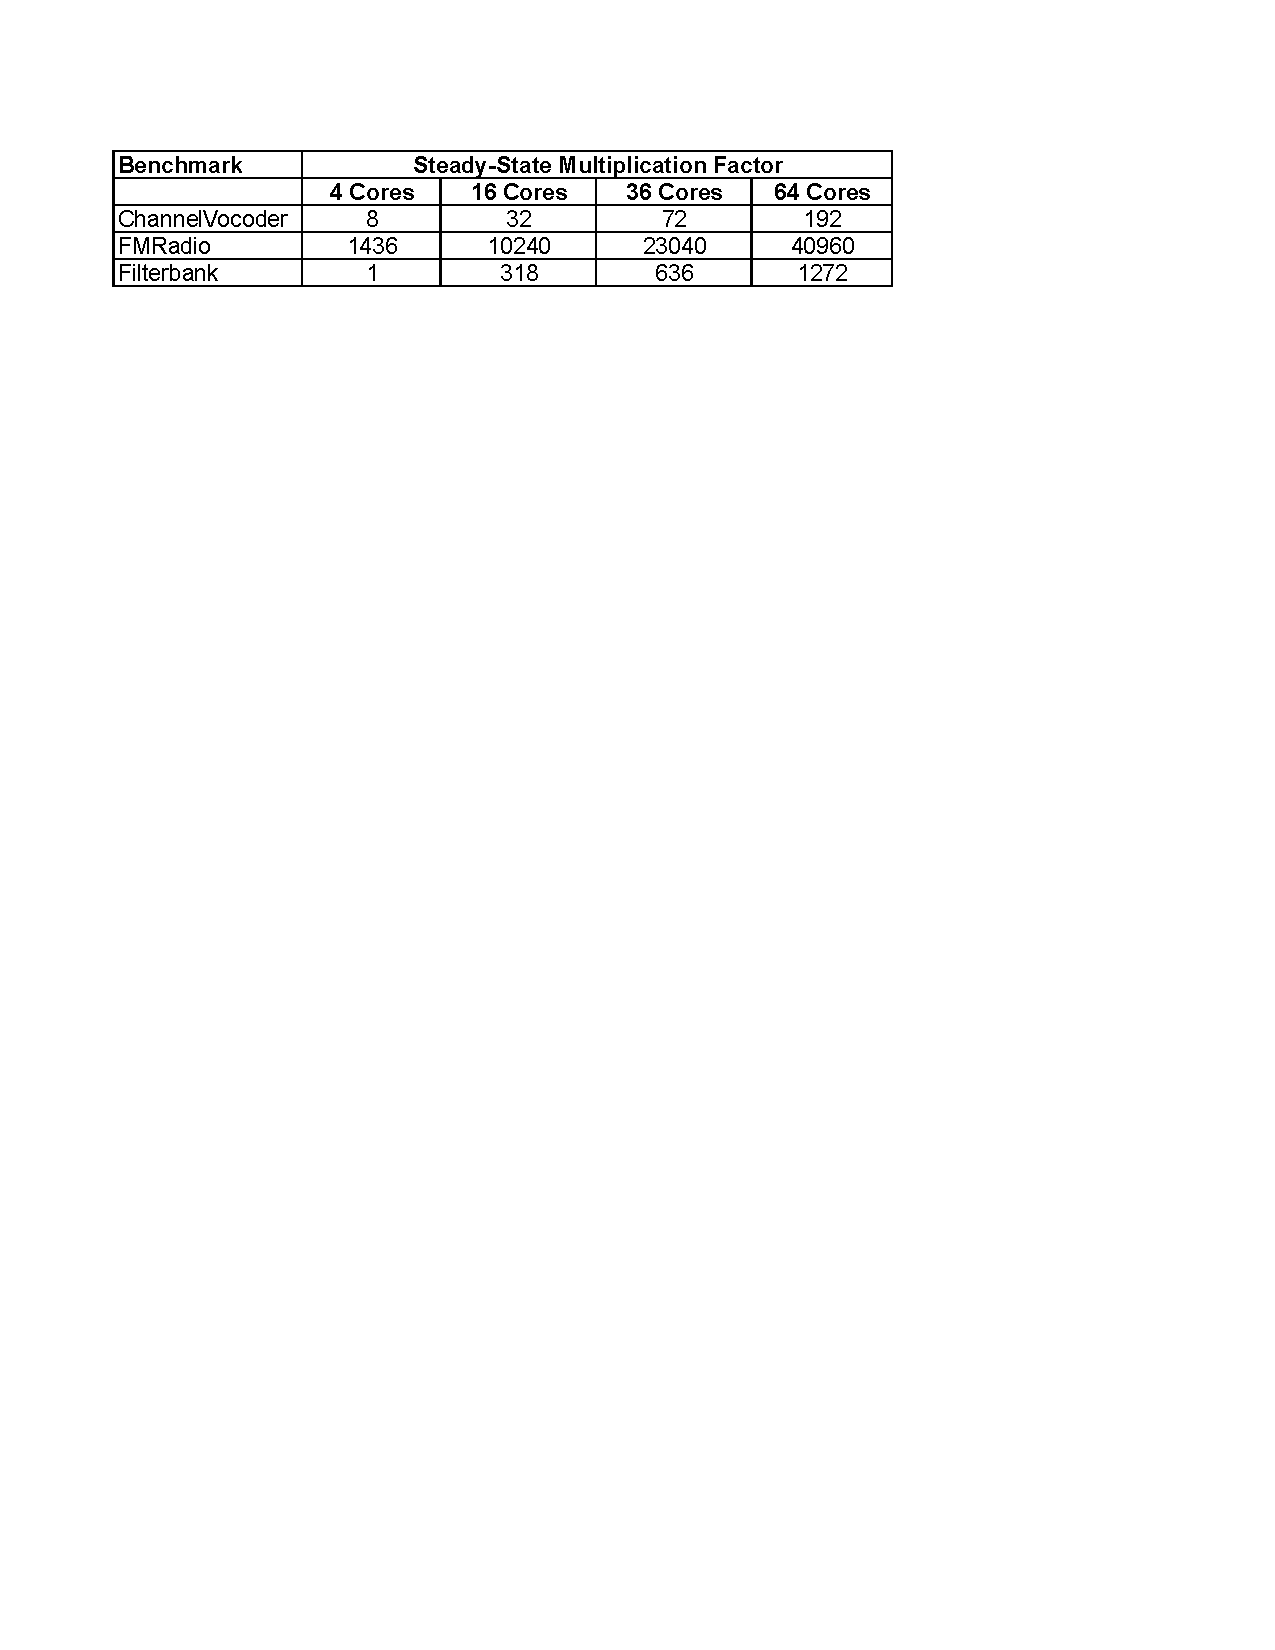
\includegraphics[width=3.7in]{figures/mult-table.pdf}} \\
% \subfigure[]{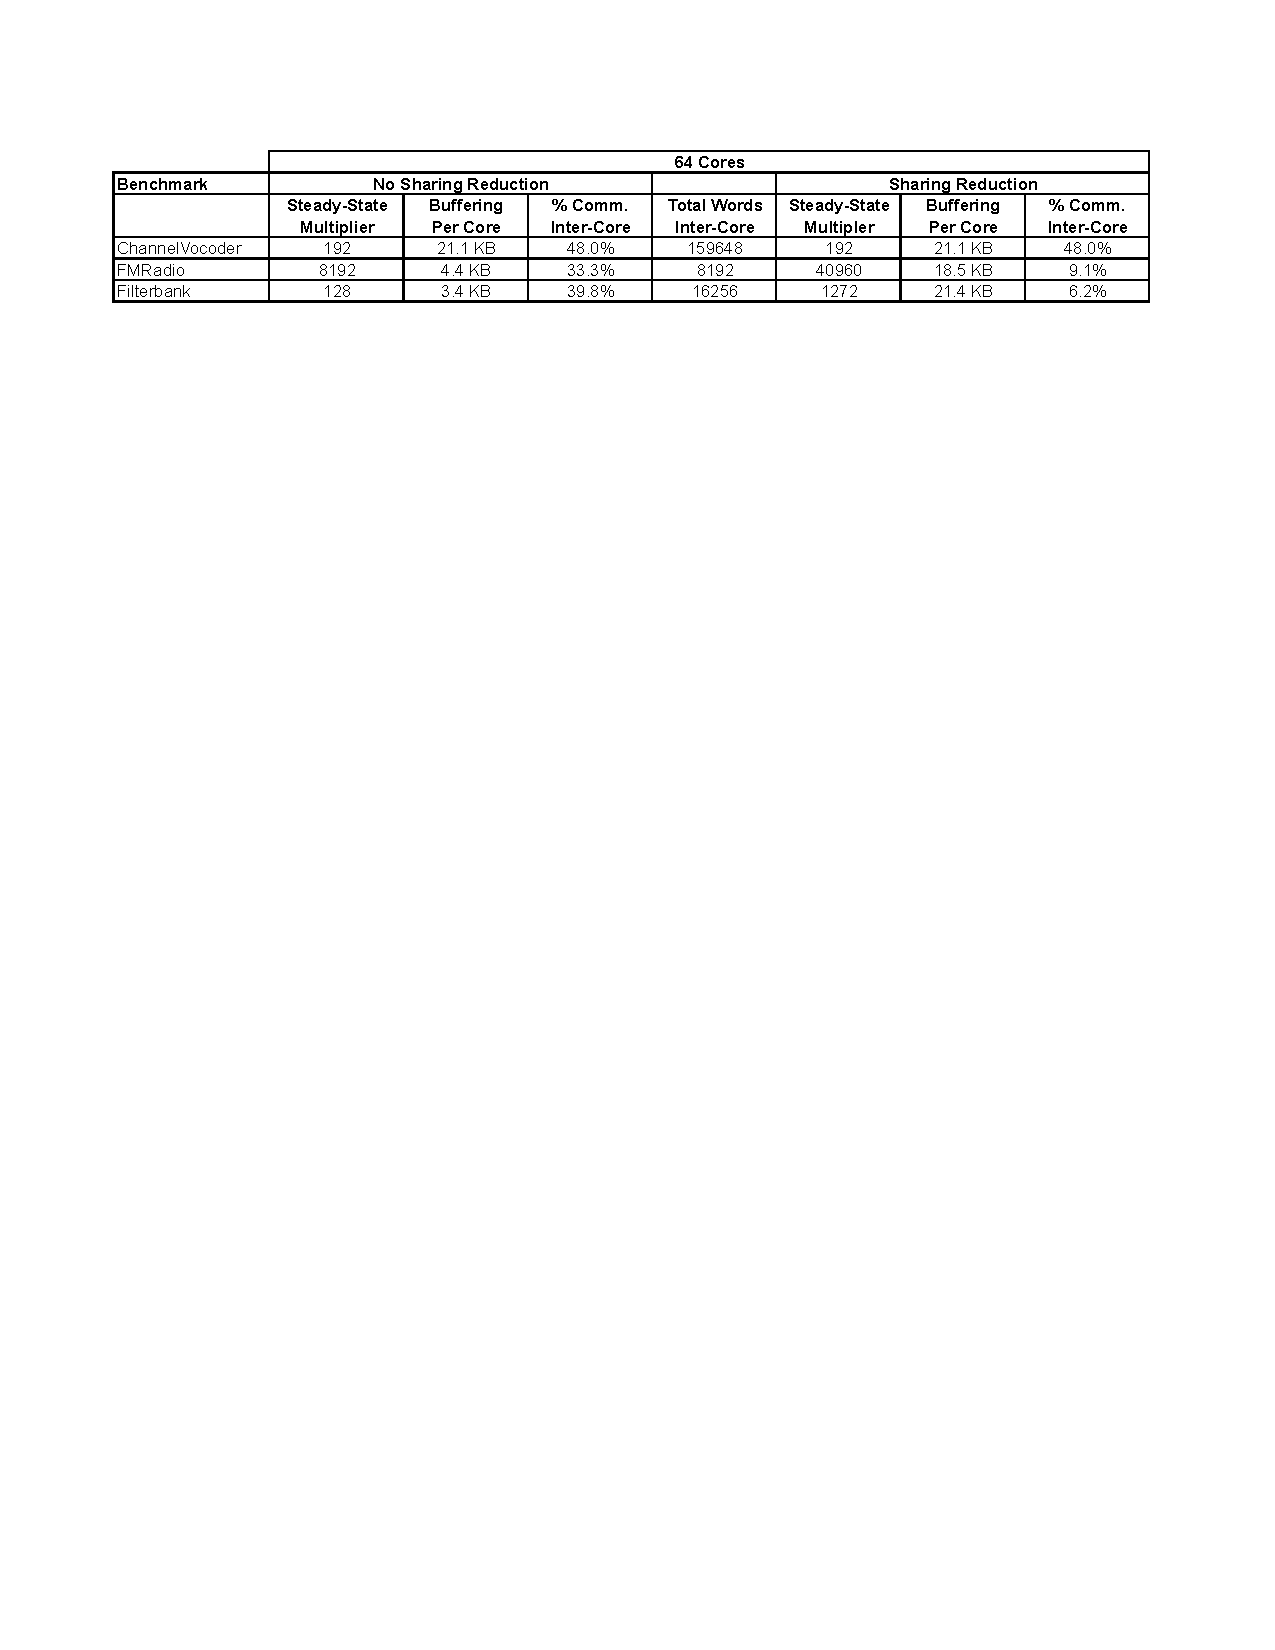
\includegraphics[width=6in]{figures/64-core-table.pdf}}
% \caption[Communication, multiplier and buffering statistics for
% benchmarks.]{
% Communication, multiplier and buffering characteristics for
% benchmarks: (a) gives the steady-state multipliers calculated for
% sharing reduction, (b) compares the steady-state with and without
% sharing reduction. 
% \label{fig:fission-table}}
% \end{figure*}

\begin{figure*}[t]
\centering
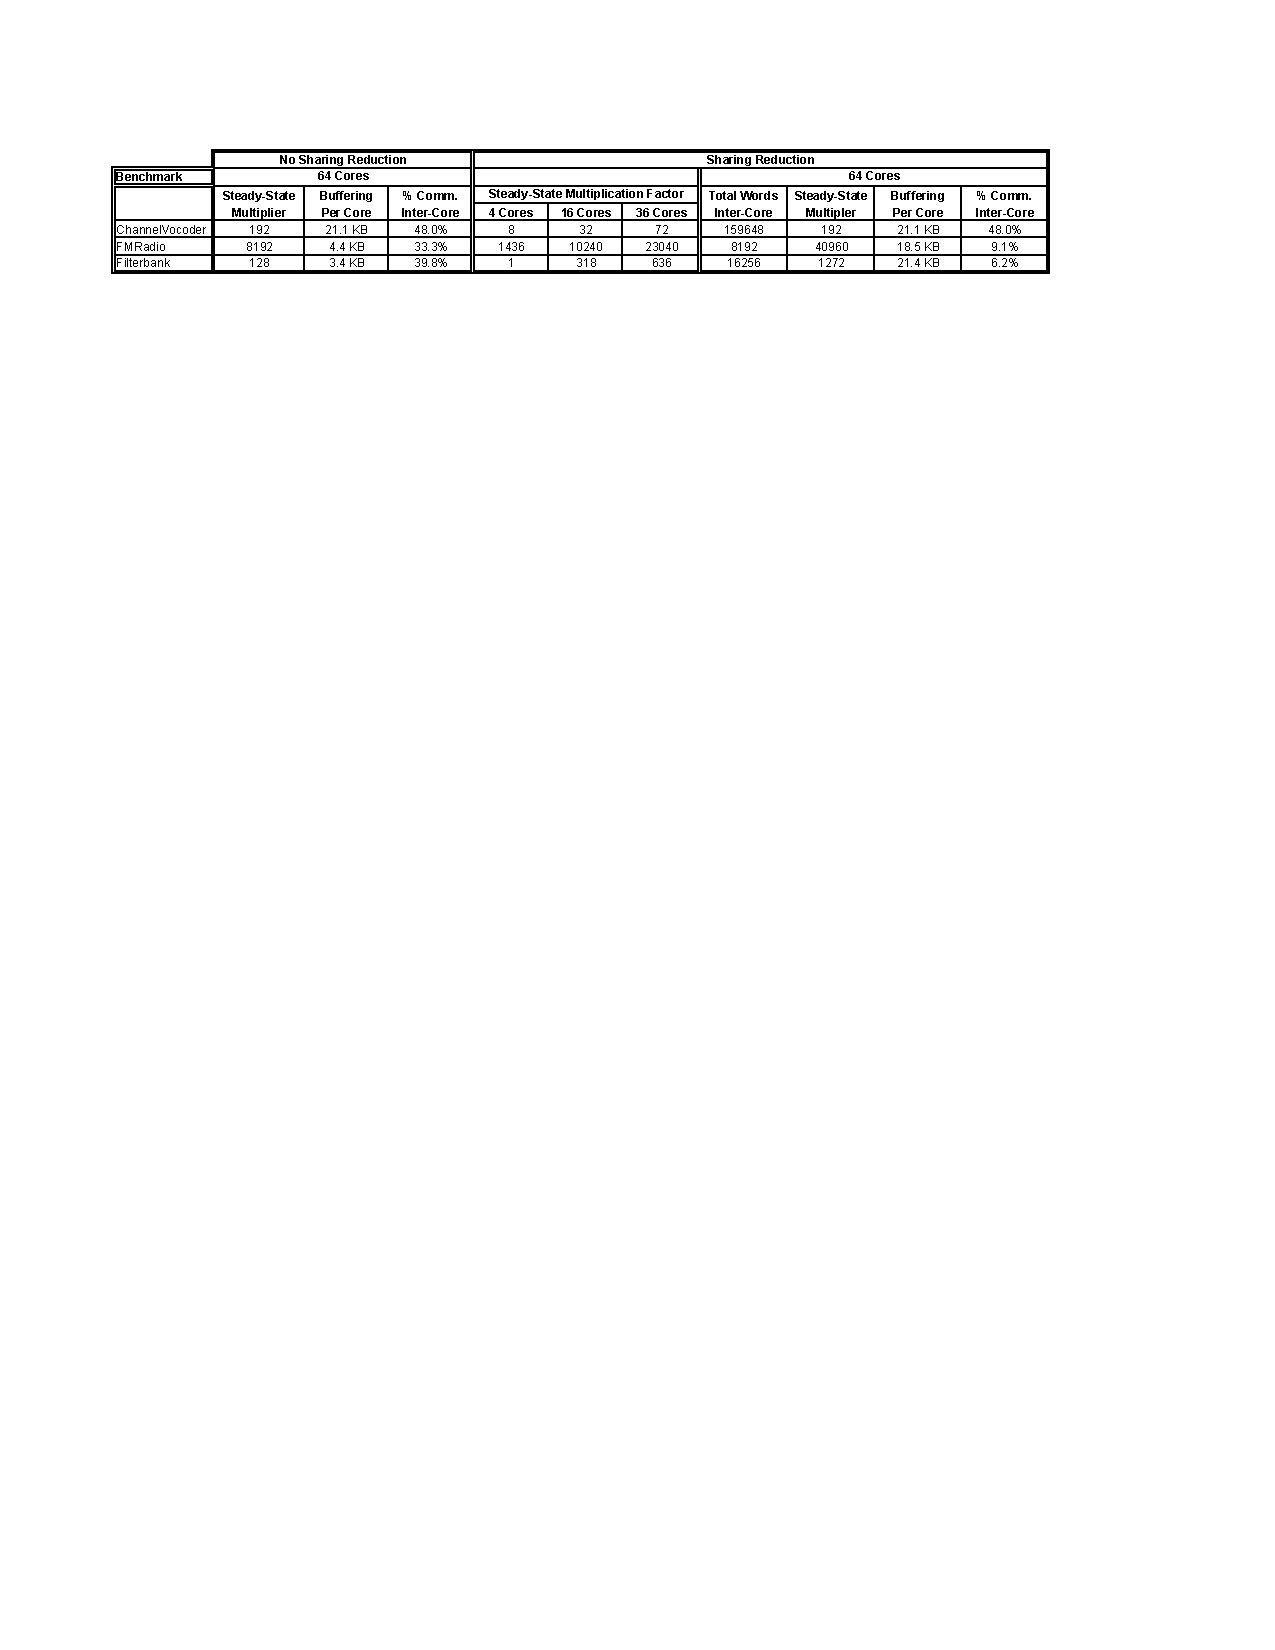
\includegraphics[width=6.1in]{figures/big-table.pdf}
\caption{\label{fig:big-table}  Steady-state multiplicity, buffering,
  and communication for fission with and without sharing reduction.}
\end{figure*}

% \begin{figure}[t]
% \centering
% 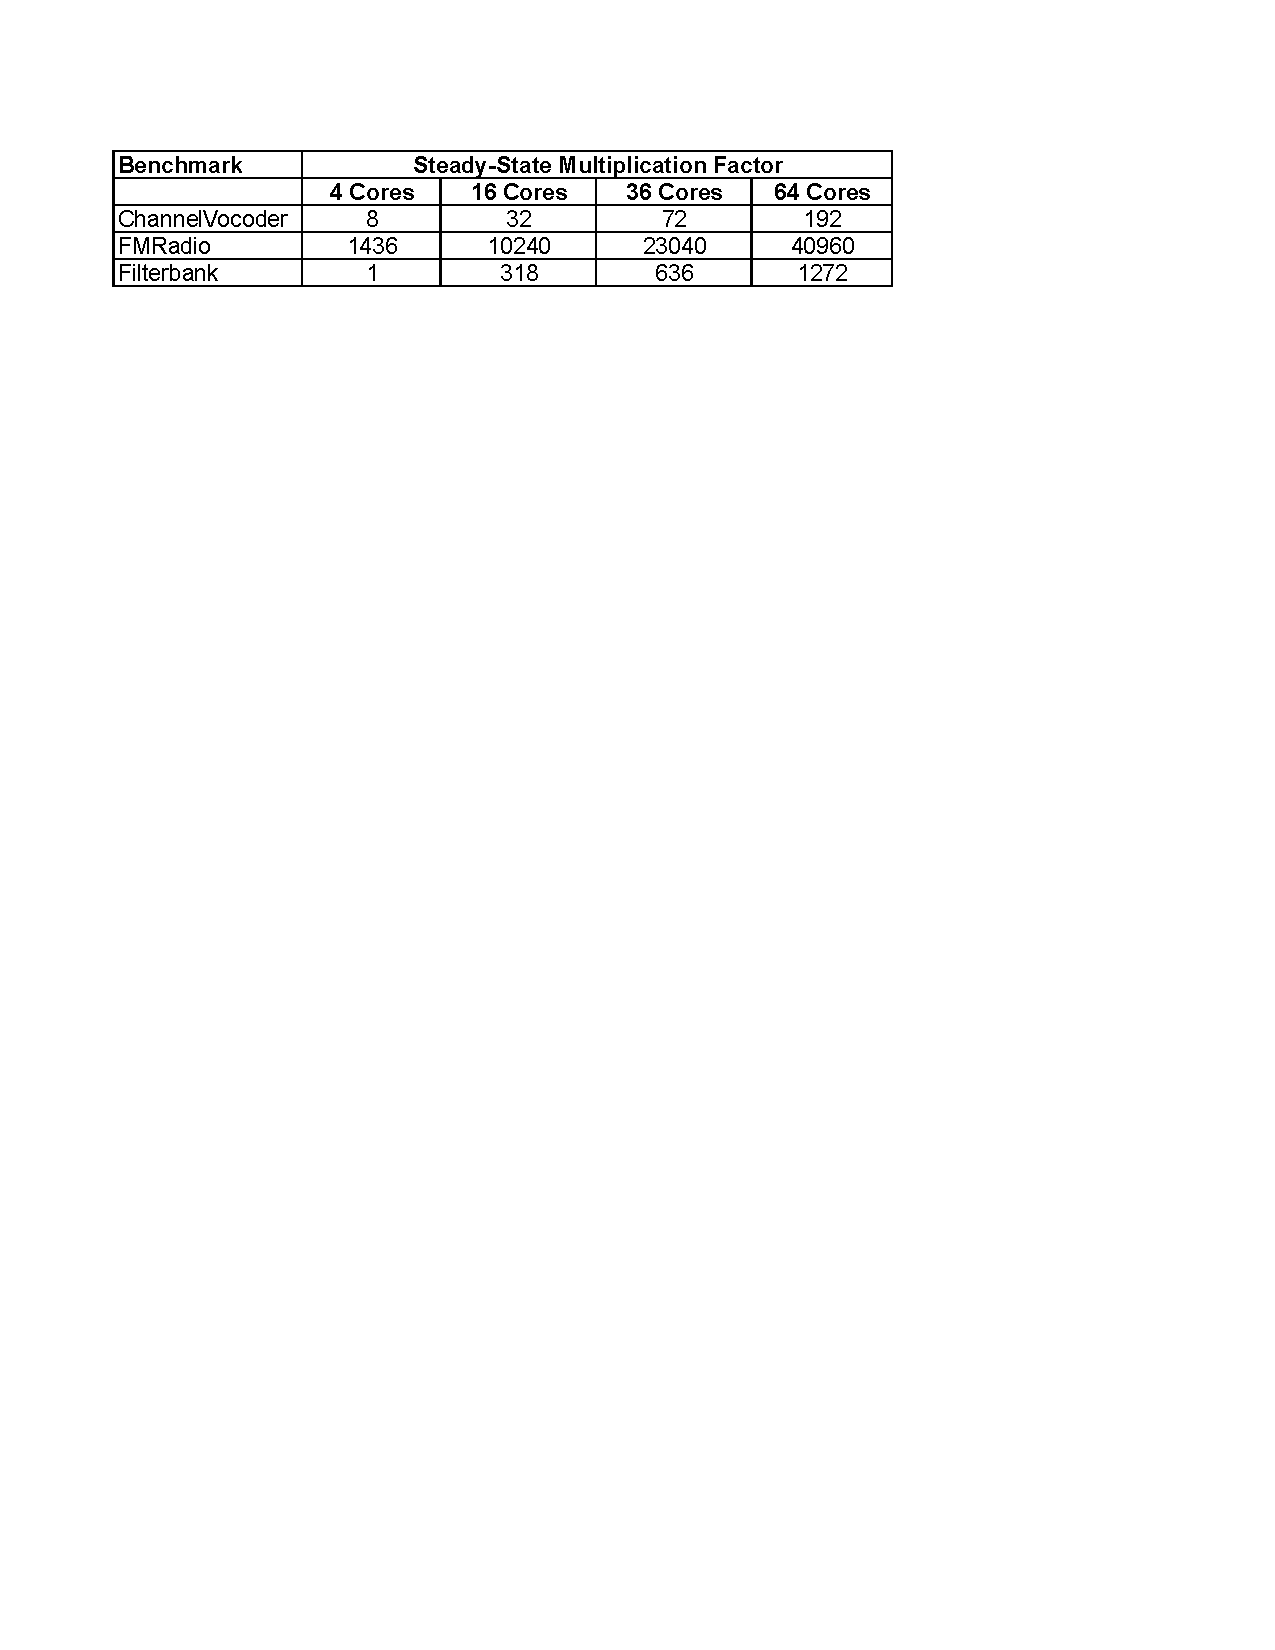
\includegraphics[width=3.3in]{figures/mult-table.pdf}
% \caption{\label{fig:mult-table}  The steady-state multipliers calculated for
% sharing reduction.}
% \end{figure}

% \begin{figure*}[t]
% \centering
% 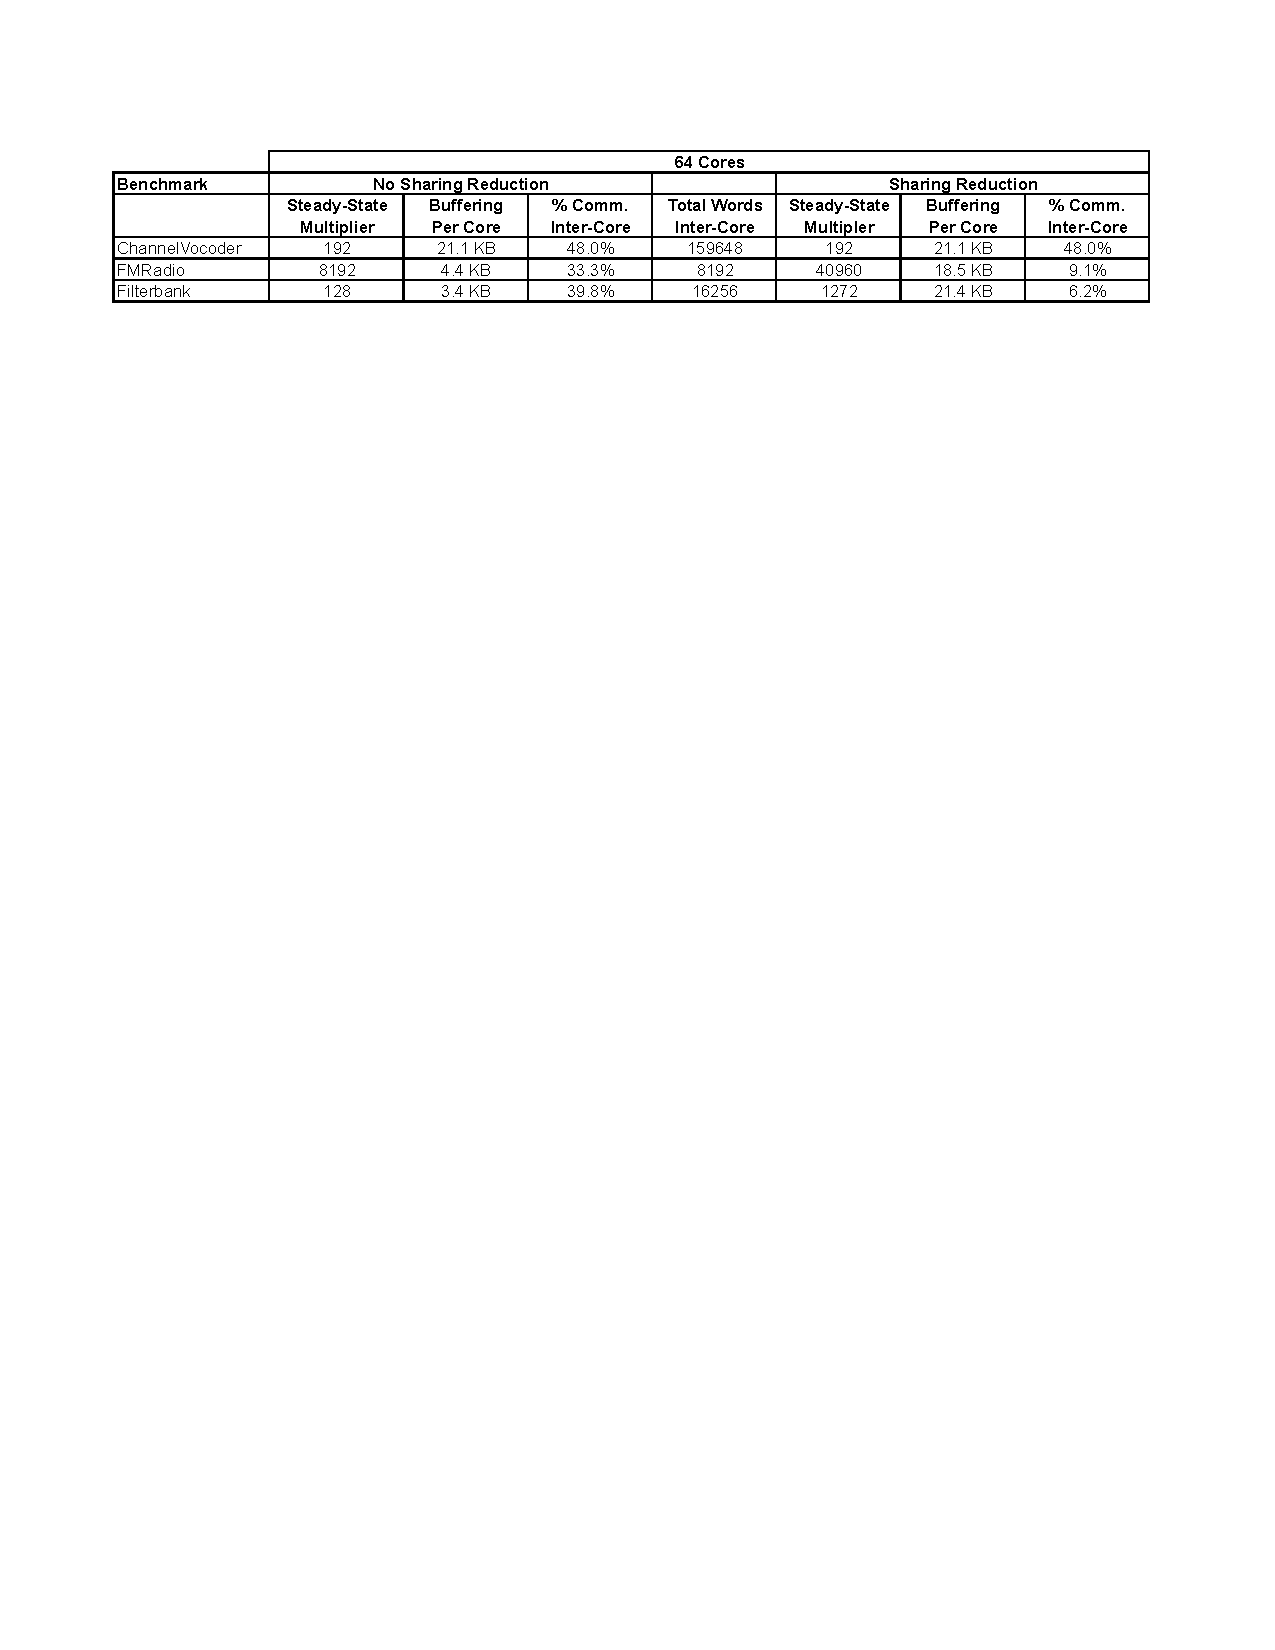
\includegraphics[width=6in]{figures/64-core-table.pdf}
% \caption{ Multiplier, buffering and communication for the steady-state with and without
% sharing reduction. 
% \label{fig:fission-table}}
% \end{figure*}

Figure~\ref{fig:big-table} compares the steady-state with and
without sharing reduction for a 64-core mapping, as well as gives the
constant $c$ calculated by sharing reduction for 4, 16, and 36.  The
factor is larger for FMRadio because one filter has $C(f) \gg o(S,
f)$.  The multiplication factor affects both latency and buffer sizes
adversely.  The application designer will have to decide if the
latency of these techniques can be borne given the application
criteria.  The total buffering requirement is increased when the
steady-state is increased.  However, since we are then fissing, the
buffer is divided amongst the fission products, and the {\it per-core}
buffering requirement is unaffected by the increase.  For example,
FMRadio, has a per-core 18 KB buffering requirement across all
configurations (4, 16, 36, and 64 cores).  This requirement fits in
the per-core L2 size of 64 KB for the Tile64.

 For ChannelVocoder,
sharing reduction has no effect because most of the peeking filters do
not satisfy $T_{\mt{apply}} = 0.05$ because of differing fission
factors between producers and consumers.  For the peeking filters that do,
the steady-state multiplier required for legal general fission for the
graph is enough to assure $T_{\mt{sharing}}$ is met.  Even though
sharing reduction has no effect for ChannelVocoder, general fission
avoids the 38\% of total items that were unnecessary duplicated by
DupDec.

For FMRadio and Filterbank, sharing reduction leads to significant
decreases in the percentage of total items communicated inter-core for
each steady-state.  The buffer requirement is increased an average of
5.2x for these benchmarks.  The total number of words communicated
inter-core during each steady-state is the same, with and without
sharing reduction.  However, the steady-state is greater in the
sharing reduction case, thus producing more outputs.

\begin{figure}[t]
\centering
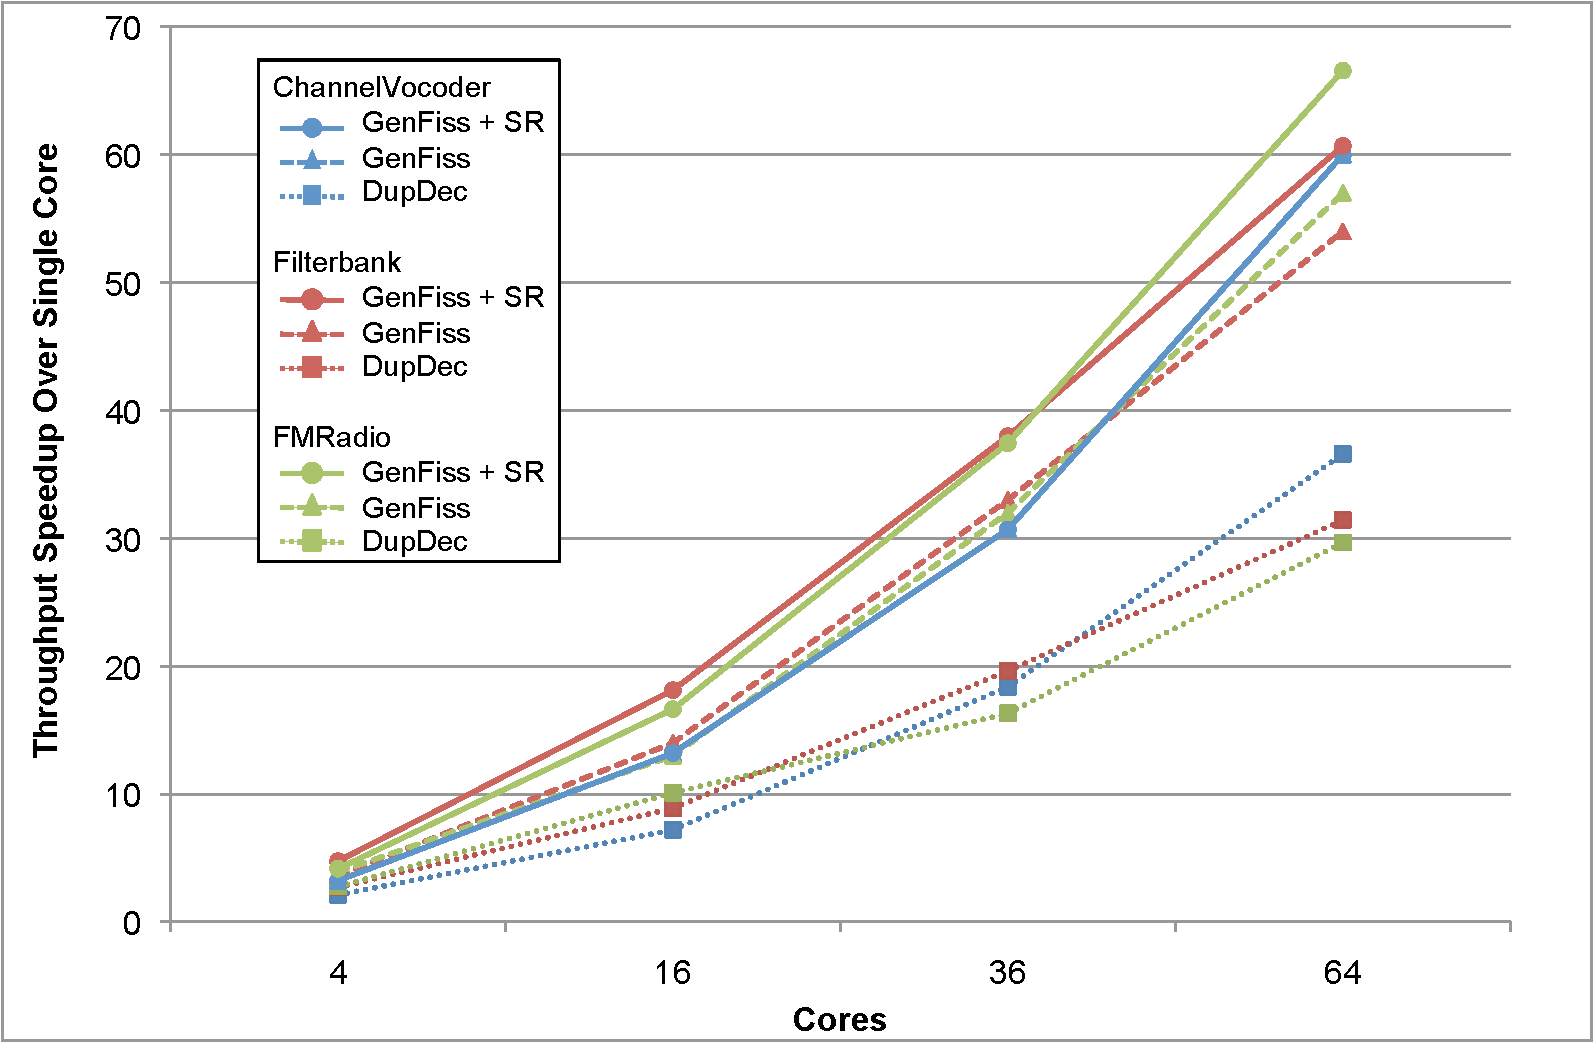
\includegraphics[width=3.3in]{figures/tilera-chart.pdf}
\caption[Comparing the fission techniques on the TILE64.]{
  Evaluation for DupDec versus general fission versus general fission with sharing reduction
  4, 16, 36, and 64 cores on the TILE64.  \label{fig:tilera-chart}}
\end{figure}

Figure~\ref{fig:tilera-chart} gives the performance results for the
Tilera TILE64 architecture.  We present results for DupDec, general
fission, and general fission with sharing reduction for 4, 16, 36, and
64 core configurations, with throughput normalized to single-core
throughput.  General fission with sharing reduction outperforms
DupDec by an average of 1.8x for the three benchmarks when targeting
64 cores. The average 64-core speedup over single core is 62.3x for the
general fission plus sharing reduction for these three benchmarks.

FMRadio experiences the most significant gain from general fission
plus sharing reduction over DupDec (67x versus 30x, respectively, for
64 cores).  FMRadio has the lowest computation to communication ratio
of the 3 benchmarks.  Furthermore, each filter of is fissed by the
number of cores targeted.  For 64 cores, each filter is fissed 64
ways.  DupDec must perform a global all-to-all communication involving
all 64 cores between each level of the graph!
 
ChannelVocoder achieves a 60x speedup for general fission over a
single core.  This is not perfectly linear because of the parallel
mapping; asymmetries exist between the extent of task parallelism and
the number of cores (see~\ref{mgordon-asplos06}).  The speedup over
DupDec (1.62x) is more modest because the width of many of the
fission applications is 3, so DupDec is duplicating input data to
groups of 3 filters.  Filterbank is similar, the width of fission is 4
for all filters when targeting 64 cores.

Sharing reduction is required to achieve scalable speedups for both
FMRadio and Filterbank.  For FMRadio, sharing reductions leads to a
17\% speedup increase for 64 cores.  This because sharing reduction
significantly reduces the number of remote write store instructions
required per output.  This affects FMRadio because of its low
computation to communication ratio.  Sharing reduction sees a 12\%
increase on Filterbank, as Filterbank has a larger computation to
communication ratio.

\begin{figure}[t]
\centering
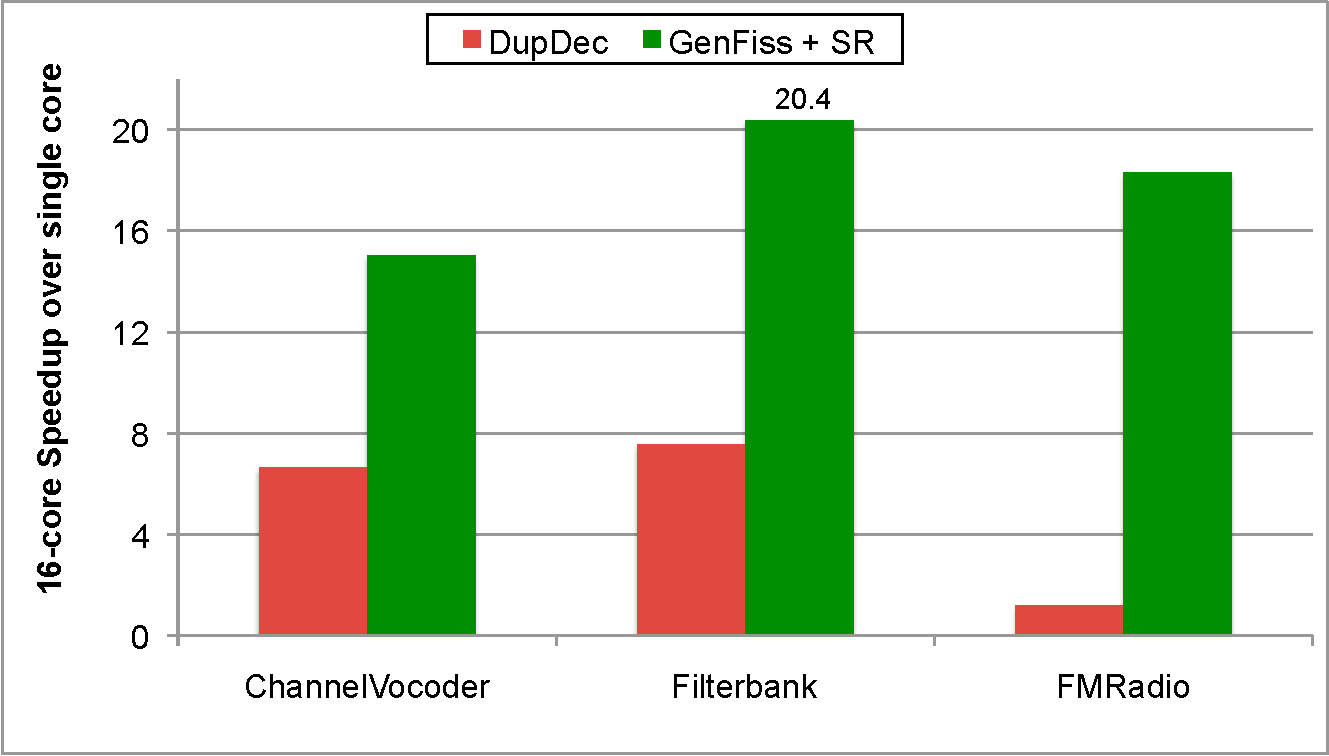
\includegraphics[width=3.3in]{figures/smp-chart.pdf}
\caption[Comparing the fission techniques on the 16-core SMP.]{
  Evaluation for DupDec versus general fission with sharing reduction
  for the 16-core SMP architecture.  \label{fig:smp-chart}}
\end{figure}

Our techniques enable scalable parallelization, with a mean speedup of
17x for our 3 benchmarks on the SMP.  Figure~\ref{fig:smp-chart} gives
the 16-core speedup comparison for DupDec versus general fission with
sharing reduction for our target SMP architecture.  The mean speedup
increase for general fission with sharing reduction over DupDec is
6.7x.  FMRadio again sees the largest speedup increase in the
comparison at 13.0x.  The reasons for this large speedup are similar
as given in the previous section.  However, the SMP communication
mechanism is not as efficient as the TILE64, thus general fission with
sharing reduction gives a greater speedup because reducing inter-core
communication has more impact.

\section{Tilera Tile64}

The TILE64 Processor, produced by Tilera Corporation, is a 64 core
system on a chip~\cite{Tilera08}.  Each core is an identical
three-wide VLIW capable of running SMP Linux.  In addition to standard
RISC instructions, all cores support a SIMD instruction set designed
to accelerate video, image and digital signal processing applications.
Each core has 64KB L2 cache, and L2 caches can be shared among cores
to provide an effective 4MB of shared L3 cache.  Cores are connected
through five low-latency, two-dimensional mesh interconnects.  Two of
these networks carry user data, while the other three handle memory
and I/O. The combination of mechanisms allows the TILE64 Processor to
support both the shared memory and message passing programming
paradigms.

%\appendix
%\section{Appendix Title}

%\acks

{
{\bibliographystyle{plainnat}
\bibliography{references}
}
}
\end{document}

